\section{Floating Point Operations}

Besides integer arithmetic, MMIX does also provide instructions to work with floating point numbers. The floating point arithmetic respects the IEEE/ANSI Standard 754. Since 64-bit quantities are the words of MMIX, arithmetic does always work with 64-bit floats, \ie "doubles". But MMIX does also support some instructions to convert from 64-bit floats to 32-bit floats and the other way around.

\subsection{Representation of Floating Point Numbers}

A 64-bit floating point number has the following structure:
\begin{figure}[H]
	\centering
	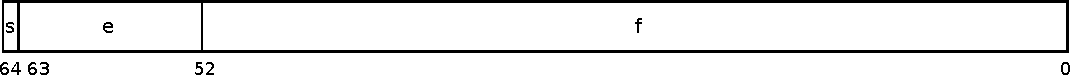
\includegraphics[width=\textwidth]{img/float-crop.pdf}
\end{figure}
\vspace{-20pt}
\noindent That means, it has a sign-bit $s$, an 11-bit exponent $e$ and a 52-bit fraction $f$. Taking $e$ as an unsigned integer and $f$ as a fraction between 0 and $(.111\dots1)_2 = 1 - 2^{-52}$, an octabyte has the following significance:
$$\vbox{\halign{\hfil$\pm#$,\quad if &#\hfil\cr
	0.0								& $e = f = 0$ (zero);\cr
	2^{\mkern1mu e - 1023}(1 + f)	& $0 < e < 2047$ (normal);\cr
	2^{-1022}f						& $e = 0$ and $f > 0$ (subnormal);\cr
	\infty							& $e = 2047$ and $f = 0$ (infinite);\cr
	\NaN(f)							& $e = 2047$ and $0 < f < 1/2$ (signaling NaN);\cr
	\NaN(f)							& $e = 2047$ and $f \ge 1/2$ (quiet NaN).\cr
}}$$
As shown, there are two representations for zero - a positive and a negative one. There are \i{normal} numbers, that can range from approximately $\pm 10^{-308}$ to $\pm 10^{308}$. Additionally \i{subnormal} numbers (also called \i{denormal} or \i{denormalized} numbers) are supported, which can range from approximately $\pm 10^{-324}$ to $\pm 10^{-308}$, but have fewer bits of precision. If the exponent has the maximum value, \ie 2047, it encodes infinity or \i{not a number} (\NaN). The latter distinguishes between \i{signaling} and \i{quiet} \NaN. Signaling \NaNs raise an invalid \glslink{Exception}{AE} when they are used, while quiet \NaNs will not. \citep[pg. 15]{mmix-doc}

Furthermore, the standard defines that four rounding modes should be available: round to nearest (and to even in case of ties, \ie the least significant bit should be zero), round off (toward zero), round up (toward $+\infty$) and round down (toward $-\infty$). MMIX uses the special register \sr{A} to specify the rounding mode. Additionally, all instructions having only one operand, specify the rounding mode with operand {\tt Y} using ${\tt Y}=0$ for the round mode in \sr{A}, ${\tt Y}=1$ for round off, ${\tt Y}=2$ for round up, ${\tt Y}=3$ for round down and ${\tt Y}=4$ for round near. \citep[pg. 15 and 21]{mmix-doc}

Last but not least, there are five kinds of \glslink{Exception}{arithmetic exceptions}, that can occur when working with floating point numbers:
\begin{enumerate}
	\item Floating overflow (value too large to be representable),
	\item Floating underflow (value too small to be representable),
	\item Floating divide by zero,
	\item Floating inexact (exact result not representable) and
	\item Floating invalid (square root of negative number, using signaling \NaN, \dots).
\end{enumerate}
As already said, all of these will either raise an \glslink{Exception}{AE} or set the corresponding \i{event bit} in \sr{A}, depending on whether the corresponding \i{enable bit} in \sr{A} is set or not. \citep[pg. 15]{mmix-doc}

\subsection{Arithmetic}

The first category of floating point operations are the arithmetic instructions. The floating point instructions don't have an \glslink{Immediate Value}{immediate} version, because it does not make much sense to specify a float with a single byte. Additionally, this section uses the notation $f(\dots)$ to indicate that a value is interpreted as a 64-bit floating point number.

\instrtbl
	{\mi{FADD|FSUB \$X,\$Y,\$Z}}
	{$\dr{X} \leftarrow f(\dr{Y}) +|- f(\dr{Z})$}
\noindent \mi{FADD} computes the sum of \dr{Y} and \dr{Z}, treating them as floating point numbers and puts the result in \dr{X}. \mi{FSUB} performs the same operation, but switches the sign of \dr{Z} first, if \dr{Z} is not \NaN. If the sum of $(+\infty)+(-\infty)$ or $(-\infty)+(+\infty)$ is computed, an invalid \glslink{Exception}{AE} will be raised. \citep[pg. 16]{mmix-doc}

\instrtbl
	{\mi{FMUL|FDIV \$X,\$Y,\$Z}}
	{$\dr{X} \leftarrow f(\dr{Y}) *|/ f(\dr{Z})$}
\noindent These instructions multiply or divide the floating point numbers \dr{Y} and \dr{Z}. Several cases result in an invalid \glslink{Exception}{AE}, like $(\pm 0.0)*(\pm \infty)$, $(\pm 0.0)/(\pm 0.0)$ or $(\pm \infty)/(\pm \infty)$. Of course, dividing by $(\pm 0.0)$ raises a floating divide by zero \glslink{Exception}{AE}. \citep[pg. 16]{mmix-doc}

\instrtbl
	{\mi{FREM \$X,\$Y,\$Z}}
	{$\dr{X} \leftarrow f(\dr{Y}) \bmod f(\dr{Z})$}
\noindent The \i{floating remainder} instruction computes the remainder and puts it into \dr{X}. This is defined "to be $\dr{Y} - n * \dr{Z}$, where $n$ is the nearest integer to $\dr{Y}/\dr{Z}$, and $n$ is an even integer in case of ties" \citep[pg. 16]{mmix-doc}. If \dr{Y} is infinite and/or \dr{Z} is zero, an invalid \glslink{Exception}{AE} will be raised. \citep[pg. 16]{mmix-doc}

\instrtbl
	{\mi{FSQRT \$X,Y,\$Z}}
	{$\dr{X} \leftarrow \sqrt{f(\dr{Z})},\quad$ using round-mode {\tt Y}}
\noindent The last one in this family is \i{floating square root}. It puts the square root of \dr{Z} into \dr{X}. An invalid \glslink{Exception}{AE} will be raised if \dr{Z} is negative, except for $-0.0$. \citep[pg. 17]{mmix-doc}

\subsection{Comparison}

Of course, besides doing arithmetic, one has to be able to compare floating point numbers. This does not work well using the integer comparison instructions, because one would have to take care of negative numbers, $+0.0$, $-0.0$ and \NaN manually. Therefore, the floating point comparisons simplify that task.

\instrtbl
	{\mi{FCMP \$X,\$Y,\$Z}}
	{$\dr{X} \leftarrow (f(\dr{Y}) > f(\dr{Z})) - (f(\dr{Y}) < f(\dr{Z}))$}
\noindent As the effect description shows, \mi{FCMP} is basically the same as \mi{CMP}, but treats the operands as floating point numbers. Thus, \dr{X} will be set to $-1$, if \dr{Y} is less than \dr{Z}, 0 if \dr{Y} is equal to \dr{Z} and 1 if \dr{Y} is greater than \dr{Z}. It will raise an invalid \glslink{Exception}{AE} and set \dr{X} to zero, if \dr{Y} or \dr{Z} is \NaN. \citep[pg. 17]{mmix-doc}

\instrtbl
	{\mi{FEQL \$X,\$Y,\$Z}}
	{$\dr{X} \leftarrow (f(\dr{Y}) = f(\dr{Z}))~?~1~:~0$}
\noindent \i{Floating equal to} sets \dr{X} to 1, if \dr{Y} and \dr{Z} are equal. But it is noteworthy, that \NaN is not equal to anything and $-0.0$ is equal to $+0.0$. \citep[pg. 17]{mmix-doc}

\instrtbl
	{\mi{FUN \$X,\$Y,\$Z}}
	{$\dr{X} \leftarrow (f(\dr{Y}) = \NaN \lor f(\dr{Z}) = \NaN)~?~1~:~0$}
\noindent The last comparison instruction is \i{floating unordered} and sets \dr{X} to 1, if \dr{Y} and \dr{Z} are considered \i{unordered}, \ie at least one of them is \NaN. \citep[pg. 17]{mmix-doc}

\subsection{Neighborhood Comparison}

Because of the limited precision of floating point numbers, operations might produce inexact results. The larger the numbers, the larger the potential difference of the produced result to the exact result. For that reason, an absolute comparison of floats, as the last section described, is not always desired. Therefore, MMIX offers another category of instructions that allow comparisons with respect to an \i{epsilon} and depending on the magnitude of the floating point numbers in question.

At first, MMIX defines a so called \i{neighborhood} of a number. Assuming that epsilon is a float called $\epsilon$, the float $u$ with fraction $f$ and exponent $e$ has the neighborhood:
\[
	N_\epsilon(u) = \left\{
	\begin{array}{l l}
		\{x \mid |x-u| \le 2^{e-1022}\epsilon\}
			& \quad \text{if $u$ is normal}\\
		\{x \mid |x-u| \le 2^{-1021}\epsilon\}
			& \quad \text{if $u$ is subnormal}\\
		\{0\}
			& \quad \text{if $u$ is zero}\\
		\{\pm \infty\}
			& \quad \text{if $u$ is $\pm \infty$ and $\epsilon < 1$}\\
		\{\text{everything except $\mp \infty$}\}
			& \quad \text{if $u$ is $\pm \infty$ and $1 \le \epsilon < 2$ and}\\
		\{\text{everything}\}
			& \quad \text{if $u$ is $\pm \infty$ and $\epsilon \ge 2$.}\\
	\end{array} \right.
\]
\citep[pg. 19]{mmix-doc} Without going into the details of this definition, it basically means that the neighborhood of a normal float depends on its exponent. That is, the larger the exponent, the larger the neighborhood.

Displayed graphically (and a bit exaggerated for demonstration purposes), the neighborhoods of a few numbers might look like the following:
\begin{figure}[H]
	\centering
	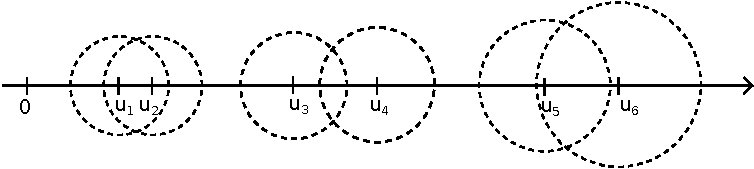
\includegraphics[width=\textwidth]{img/cmpe-less-crop.pdf}
	\caption{Example neighborhoods, demonstrating float relationships}
\end{figure}
\noindent MMIX distinguishes four cases when comparing floats $u$ and $v$ with respect to $\epsilon$:
\begin{enumerate}
	\item $u \approx v$, if $u \in N_\epsilon(v)$ and $v \in N_\epsilon(u)$.\\
	That means, two numbers will be considered \i{equivalent}, if both are in the neighborhood of the corresponding other number. In the example, only $u_1 \approx u_2$, because $u_1 \in N_\epsilon(u_2)$ and $u_2 \in N_\epsilon(u_1)$.
	\item $u \sim v$, if $u \in N_\epsilon(v)$ or $v \in N_\epsilon(u)$.\\
	Thus, two numbers will be considered \i{similar}, if only one of them belongs to the neighborhood of the corresponding other number. For example, $u_5 \sim u_6$, because $u_5 \in N_\epsilon(u_6)$, but $u_6 \notin N_\epsilon(u_5)$.
	\item $u \prec v$, if $u < N_\epsilon(v)$ and $N_\epsilon(u) < v$.\\
	For example, $u_3 \prec u_4$ because $u_3$ is less than all numbers in $N_\epsilon(u_4)$ and all numbers in $N_\epsilon(u_3)$ are less than $u_4$.
	\item $u \succ v$, if $u > N_\epsilon(v)$ and $N_\epsilon(u) > v$.\\
	Analogous, $u_4 \succ u_3$.
\end{enumerate}
\citep[pg. 19]{mmix-doc} The following instructions are based on this definition and use the special \i{epsilon register} \sr{E} for $\epsilon$.

\instrtbl
	{\mi{FCMPE \$X,\$Y,\$Z}}
	{$\dr{X} \leftarrow (f(\dr{Y}) \succ f(\dr{Z})~(\sr{E})) - (f(\dr{Y}) \prec f(\dr{Z})~(\sr{E}))$}
\noindent Analogous to \mi{FCMP}, \mi{FCMPE} -- called \i{floating compare with respect to epsilon} -- compares \dr{Y} with \dr{Z} according to the definition above and sets \dr{X} to $-1$, 0 or 1. It should be noted, that \dr{X} will be set to zero, if \dr{Y} is similar \i{or} equivalent to \dr{Z}. An invalid \glslink{Exception}{AE} will be raised, if \dr{Y}, \dr{Z} or \sr{E} is \NaN or \sr{E} is negative. \citep[pg. 19]{mmix-doc}

\instrtbl
	{\mi{FEQLE \$X,\$Y,\$Z}}
	{$\dr{X} \leftarrow (f(\dr{Y}) \approx f(\dr{Z})~(\sr{E}))~?~1~:~0$}
\noindent Similarly to \mi{FEQL}, \mi{FEQLE} will set \dr{X} to 1, if \dr{Y} is equivalent to \dr{Z}, depending on \sr{E}. It raises the same \glslink{Exception}{arithmetic exceptions} as \mi{FCMPE}. \citep[pg. 19]{mmix-doc}

\instrtbl
	{\mi{FUNE \$X,\$Y,\$Z}}
	{$\dr{X} \leftarrow (f(\dr{Y}) = \NaN \lor f(\dr{Z}) = \NaN \lor \sr{E} = \NaN \lor \sr{E} < 0)~?~1~:~0$}
\noindent The last one in this group is \mi{FUNE}, which will set \dr{X} to 1, if \dr{Y}, \dr{Z} or \sr{E} are exceptional as described for \mi{FCMPE} and \mi{FEQLE}. \citep[pg. 19]{mmix-doc}

\subsection{Conversion between Float and Integer}

MMIX offers three groups of instructions to convert an integer to a floating point number and the other way around.

\instrtbl
	{\mi{FIX|FIXU \$X,Y,\$Z}}
	{$\dr{X} \leftarrow (int)f(\dr{Z}) \bmod 2^{64},\quad$ using round-mode {\tt Y}}
\noindent The instructions \i{convert floating to fixed} and \i{convert floating to fixed unsigned} take \dr{Z} as a float, convert it to an integer and put it into \dr{X}. Only when using \mi{FIX}, an invalid \glslink{Exception}{AE} will be raised if \dr{Z} is infinite or \NaN and a float-to-fix \glslink{Exception}{AE} will occur, if the result is less than $-2^{63}$ or greater than $2^{63}-1$. \citep[pg. 20]{mmix-doc}

\instrtbl
	{\mi{FINT \$X,Y,\$Z}}
	{$\dr{X} \leftarrow f((int)f(\dr{Z})),\quad$ using round-mode {\tt Y}}
\noindent The instruction \i{floating integer} rounds the float \dr{Z} to a floating integer and places it in \dr{X}. Infinity and \NaN are not changed. The difference to \mi{FIX} is, that \mi{FINT} writes a floating point number to \dr{X}, while \mi{FIX} writes a signed integer to \dr{X}. \citep[pg. 17]{mmix-doc}

\instrtbl
	{\mi{FLOT|FLOTU \$X,Y,\$Z|Z}}
	{$\dr{X} \leftarrow f(\sdrimm{Z}),\quad$ using round-mode {\tt Y}}
\noindent Finally, the instructions \i{convert fixed to floating} and \i{convert fixed to floating unsigned} treat \udrim{Z} as an integer and convert it to the nearest floating point number. Only if using \mi{FLOT}, an floating inexact \glslink{Exception}{AE} will be raised, if rounding is necessary. \citep[pg. 20]{mmix-doc}

\subsection{Short Floats}

Although MMIX is a 64-bit architecture and thus, works with 64-bit floating point values by default, it does also provide some instructions to use 32-bit floating point numbers, called \i{short floats}. But MMIX has no separate arithmetic or comparison instructions for them. Instead it offers instructions to load a short float from memory into a float and store a float as a short float to memory.

\instrtbl
	{\mi{LDSF \$X,\$Y,\$Z|Z}}
	{$\dr{X} \leftarrow f(sf(\vmem{4}{\dr{Y} + \udrim{Z}}))$}
\noindent The first one, called \i{load short float}, loads the tetra \vmem{4}{\dr{Y} + \udrim{Z}}, treating it as a 32-bit float, converts it to a 64-bit float and puts it into \dr{X}. \citep[pg. 20]{mmix-doc}

\instrtbl
	{\mi{STSF \$X,\$Y,\$Z|Z}}
	{$\vmem{4}{\dr{Y} + \udrim{Z}}~\leftarrow sf(f(\dr{X}))$}
\noindent \mi{STSF} goes the other way: it treats \dr{X} as a 64-bit float, converts it to a 32-bit float and stores that into \vmem{4}{\dr{Y} + \udrim{Z}}. It may trigger a floating overflow, underflow, inexact and invalid \glslink{Exception}{AE}. \citep[pg. 20]{mmix-doc}

\instrtbl
	{\mi{SFLOT|SFLOTU \$X,Y,\$Z|Z}}
	{$\dr{X} \leftarrow f(sf(\sdrimm{Z})),\quad$ using round-mode {\tt Y}}
\noindent These instructions behave like \mi{FLOT} and \mi{FLOTU}, but convert \sdrim{Z} to a 32-bit float first, which ensures that no \glslink{Exception}{AE} will be raised if \dr{X} is stored with \mi{STSF} afterwards. \citep[pg. 20]{mmix-doc}


